\ifdefined\pdfminorversion\pdfminorversion=7\fi
%% LocalGuard -- WSDM 2027 short paper (anonymous, review mode)
\documentclass[sigconf,anonymous,review,balance=false]{acmart}
\usepackage{amsmath}
\usepackage{booktabs}
\usepackage{tikz,pifont}
\copyrightyear{2027}\acmYear{2027}\setcopyright{acmlicensed}
\acmConference[WSDM '27]{Proceedings of the 20th ACM International Conference
  on Web Search and Data Mining}{February 15--19, 2027}{}
\acmBooktitle{Proceedings of the 20th ACM International Conference on Web
  Search and Data Mining (WSDM '27)}
\acmSubmissionID{109}\acmDOI{}\acmISBN{}
\newcommand{\system}{LocalGuard}
\newtheorem{proposition}{Proposition}
\newcommand{\MeanRatingUtility}{0.893}
\newcommand{\MeanRatingKept}{27\% [1, 48]}
\newcommand{\MeanRatingDelta}{-0.029 [-0.041, -0.017]}
\newcommand{\SecondJudgeGain}{-0.006 [-0.031, +0.022]}
\newcommand{\SecondJudgeQwenGain}{+0.016 [-0.005, +0.040]}
\newcommand{\CumulativeSingleOne}{0.375}
\newcommand{\CumulativeSingleTen}{0.490}
\newcommand{\CumulativeCalibratedTen}{0.351}
\newcommand{\qaCountLoss}{0.107}
\newcommand{\qaCountSize}{2.18}
\newcommand{\qaWeightedLoss}{0.086}
\newcommand{\qaWeightedSize}{1.28}
\newcommand{\threeCountLoss}{0.150}
\newcommand{\threeCountSize}{3.11}
\newcommand{\threeWeightedLoss}{0.090}
\newcommand{\threeWeightedSize}{1.98}
\newcommand{\sevenCountLoss}{0.000}
\newcommand{\sevenCountSize}{0.00}
\newcommand{\sevenWeightedLoss}{0.000}
\newcommand{\sevenWeightedSize}{0.00}
\newcommand{\qaNEval}{300}
\newcommand{\qaNReader}{150}
\newcommand{\qaRateDisc}{18}
\newcommand{\qaRateGemma}{23}
\newcommand{\qaRateUnion}{26}
\newcommand{\qaKappaFull}{0.66}
\newcommand{\qaRateSensUnion}{8}
\newcommand{\qaQwenRecGemma}{65}
\newcommand{\qaUsersAnyUnion}{77}
\newcommand{\qaDetRecallUnion}{62}
\newcommand{\qaNecSpearman}{0.01}
\newcommand{\qaUNone}{0.608}
\newcommand{\qaUSimK}{0.624}
\newcommand{\qaESimK}{1.41}
\newcommand{\qaESimKQwen}{0.93}
\newcommand{\qaESimKAny}{73}
\newcommand{\qaESimKSens}{0.41}
\newcommand{\qaTopFiveGain}{+0.016 [-0.008, +0.039]}
\newcommand{\qaRandKept}{-111}
\newcommand{\qaFixMedExpo}{0.33}
\newcommand{\qaFixMedSize}{3.6}
\newcommand{\qaFixMedUtil}{0.617}
\newcommand{\qaCalQwenMeasQwen}{0}
\newcommand{\qaCalQwenMeasQwenWorst}{-0.03}
\newcommand{\qaCalQwenMeasGemma}{54}
\newcommand{\qaCalQwenMeasGemmaWorst}{+0.16}
\newcommand{\qaCalQwenMeasUnion}{67}
\newcommand{\qaCalQwenMeasUnionWorst}{+0.33}
\newcommand{\qaCalQwenMeasUnionAny}{50}
\newcommand{\qaCalQwenMeasUnionAnyWorst}{+0.15}
\newcommand{\qaCalQwenMeasUnionSens}{29}
\newcommand{\qaCalQwenMeasUnionSensWorst}{+0.07}
\newcommand{\qaCalUnionMeasQwen}{0}
\newcommand{\qaCalUnionMeasQwenWorst}{-0.08}
\newcommand{\qaCalUnionMeasGemma}{0}
\newcommand{\qaCalUnionMeasGemmaWorst}{-0.05}
\newcommand{\qaCalUnionMeasUnion}{0}
\newcommand{\qaCalUnionMeasUnionWorst}{-0.04}
\newcommand{\qaCalUnionMeasUnionAny}{0}
\newcommand{\qaCalUnionMeasUnionAnyWorst}{-0.01}
\newcommand{\qaCalUnionMeasUnionSens}{0}
\newcommand{\qaCalUnionMeasUnionSensWorst}{-0.03}
\newcommand{\qaAnyCSimB}{0.10}
\newcommand{\qaSensCSimB}{0.11}
\newcommand{\qaAnyCSimD}{0.39}
\newcommand{\qaSensCSimD}{0.38}
\newcommand{\qaSimExpoB}{0.00}
\newcommand{\qaSimUtilB}{0.608}
\newcommand{\qaSimSizeB}{0.0}
\newcommand{\qaSimVsTopB}{-0.015 [-0.035, +0.003]}
\newcommand{\qaSimVsNoneB}{+0.000 [+0.000, +0.000]}
\newcommand{\qaLttSimExpoB}{0.00}
\newcommand{\qaLttSimUtilB}{0.608}
\newcommand{\qaLttSimSizeB}{0.0}
\newcommand{\qaLttSimVsTopB}{-0.015 [-0.035, +0.003]}
\newcommand{\qaLttSimVsNoneB}{+0.000 [+0.000, +0.000]}
\newcommand{\qaSimThrExpoB}{0.21}
\newcommand{\qaSimThrUtilB}{0.609}
\newcommand{\qaSimThrSizeB}{0.5}
\newcommand{\qaSimThrVsTopB}{-0.015 [-0.034, +0.004]}
\newcommand{\qaSimThrVsNoneB}{+0.000 [-0.014, +0.014]}
\newcommand{\qaLttSimThrExpoB}{0.04}
\newcommand{\qaLttSimThrUtilB}{0.609}
\newcommand{\qaLttSimThrSizeB}{0.1}
\newcommand{\qaLttSimThrVsTopB}{-0.014 [-0.034, +0.005]}
\newcommand{\qaLttSimThrVsNoneB}{+0.002 [-0.005, +0.010]}
\newcommand{\qaFltExpoB}{0.02}
\newcommand{\qaFltUtilB}{0.607}
\newcommand{\qaFltSizeB}{0.1}
\newcommand{\qaFltVsTopB}{-0.017 [-0.037, +0.004]}
\newcommand{\qaFltVsNoneB}{-0.001 [-0.017, +0.011]}
\newcommand{\qaLttFltExpoB}{0.00}
\newcommand{\qaLttFltUtilB}{0.608}
\newcommand{\qaLttFltSizeB}{0.0}
\newcommand{\qaLttFltVsTopB}{-0.015 [-0.035, +0.003]}
\newcommand{\qaLttFltVsNoneB}{+0.000 [+0.000, +0.000]}
\newcommand{\qaCSimExpoB}{0.13}
\newcommand{\qaCSimUtilB}{0.628}
\newcommand{\qaCSimSizeB}{2.2}
\newcommand{\qaCSimVsTopB}{+0.004 [-0.015, +0.023]}
\newcommand{\qaCSimVsNoneB}{+0.019 [-0.005, +0.043]}
\newcommand{\qaLttCSimExpoB}{0.00}
\newcommand{\qaLttCSimUtilB}{0.608}
\newcommand{\qaLttCSimSizeB}{0.0}
\newcommand{\qaLttCSimVsTopB}{-0.014 [-0.032, +0.006]}
\newcommand{\qaLttCSimVsNoneB}{+0.001 [+0.000, +0.017]}
\newcommand{\qaNSigLossB}{0}
\newcommand{\qaNSigGainB}{0}
\newcommand{\qaNNonInfB}{0}
\newcommand{\qaSimExpoD}{0.34}
\newcommand{\qaSimUtilD}{0.606}
\newcommand{\qaSimSizeD}{1.0}
\newcommand{\qaSimVsTopD}{-0.019 [-0.038, -0.000]}
\newcommand{\qaSimVsNoneD}{-0.003 [-0.028, +0.020]}
\newcommand{\qaLttSimExpoD}{0.16}
\newcommand{\qaLttSimUtilD}{0.607}
\newcommand{\qaLttSimSizeD}{0.5}
\newcommand{\qaLttSimVsTopD}{-0.017 [-0.036, +0.004]}
\newcommand{\qaLttSimVsNoneD}{-0.001 [-0.022, +0.016]}
\newcommand{\qaSimThrExpoD}{0.50}
\newcommand{\qaSimThrUtilD}{0.610}
\newcommand{\qaSimThrSizeD}{1.6}
\newcommand{\qaSimThrVsTopD}{-0.013 [-0.030, +0.002]}
\newcommand{\qaSimThrVsNoneD}{+0.002 [-0.016, +0.024]}
\newcommand{\qaLttSimThrExpoD}{0.30}
\newcommand{\qaLttSimThrUtilD}{0.606}
\newcommand{\qaLttSimThrSizeD}{0.9}
\newcommand{\qaLttSimThrVsTopD}{-0.017 [-0.034, +0.002]}
\newcommand{\qaLttSimThrVsNoneD}{-0.001 [-0.017, +0.015]}
\newcommand{\qaFltExpoD}{0.35}
\newcommand{\qaFltUtilD}{0.598}
\newcommand{\qaFltSizeD}{1.9}
\newcommand{\qaFltVsTopD}{-0.026 [-0.046, -0.008]}
\newcommand{\qaFltVsNoneD}{-0.011 [-0.036, +0.012]}
\newcommand{\qaLttFltExpoD}{0.19}
\newcommand{\qaLttFltUtilD}{0.600}
\newcommand{\qaLttFltSizeD}{1.0}
\newcommand{\qaLttFltVsTopD}{-0.024 [-0.044, -0.005]}
\newcommand{\qaLttFltVsNoneD}{-0.008 [-0.030, +0.012]}
\newcommand{\qaCSimExpoD}{0.42}
\newcommand{\qaCSimUtilD}{0.614}
\newcommand{\qaCSimSizeD}{4.1}
\newcommand{\qaCSimVsTopD}{-0.010 [-0.027, +0.008]}
\newcommand{\qaCSimVsNoneD}{+0.006 [-0.017, +0.030]}
\newcommand{\qaLttCSimExpoD}{0.18}
\newcommand{\qaLttCSimUtilD}{0.625}
\newcommand{\qaLttCSimSizeD}{2.5}
\newcommand{\qaLttCSimVsTopD}{+0.001 [-0.021, +0.021]}
\newcommand{\qaLttCSimVsNoneD}{+0.016 [-0.009, +0.041]}
\newcommand{\qaNSigLossD}{2}
\newcommand{\qaNSigGainD}{0}
\newcommand{\qaNNonInfD}{0}
\newcommand{\qaQcalCSimUtilB}{0.616}
\newcommand{\qaQcalCSimExpoB}{0.35}
\newcommand{\qaQcalCSimUtilD}{0.615}
\newcommand{\qaQcalCSimExpoD}{0.74}
\newcommand{\qaShiftMain}{0.14}
\newcommand{\qaShiftNec}{0.17}
\newcommand{\qaShiftMainFrac}{8}
\newcommand{\qaShiftRand}{0.04}
\newcommand{\qaMonPooled}{-0.010}
\newcommand{\qaMonMondrian}{-0.059}
\newcommand{\qaOrExpo}{0.06}
\newcommand{\qaOrSuff}{99}
\newcommand{\qaOrEmpty}{70}
\newcommand{\qaOrEmptyCI}{70\% [60, 79]}
\newcommand{\qaOrSimKGap}{1.19}
\newcommand{\qaOrSimKGapCI}{1.19 [0.95, 1.44]}
\newcommand{\qaOrNeeds}{6}
\newcommand{\qaOrNeedsCI}{6\% [1, 11]}
\newcommand{\qaOrN}{80}
\newcommand{\qaShiftNecNoFeat}{0.04}
\newcommand{\qaOrSimKExpo}{1.25}
\newcommand{\qaFixLttDep}{0}
\newcommand{\qaFixCrcDepTopOne}{0}
\newcommand{\qaFixCrcTopOneUtil}{0.607}
\newcommand{\qaFixLttDepTopOne}{0}
\newcommand{\threeNEval}{450}
\newcommand{\threeNReader}{450}
\newcommand{\threeRateDisc}{12}
\newcommand{\threeRateGemma}{16}
\newcommand{\threeRateUnion}{18}
\newcommand{\threeKappaFull}{0.67}
\newcommand{\threeRateSensUnion}{3}
\newcommand{\threeQwenRecGemma}{63}
\newcommand{\threeUsersAnyUnion}{60}
\newcommand{\threeDetRecallUnion}{55}
\newcommand{\threeNecSpearman}{0.05}
\newcommand{\threeUNone}{0.883}
\newcommand{\threeUSimK}{0.922}
\newcommand{\threeESimK}{0.94}
\newcommand{\threeESimKQwen}{0.63}
\newcommand{\threeESimKAny}{48}
\newcommand{\threeESimKSens}{0.14}
\newcommand{\threeTopFiveGain}{+0.039 [+0.023, +0.055]}
\newcommand{\threeRandKept}{65}
\newcommand{\threeFixMedExpo}{0.15}
\newcommand{\threeFixMedSize}{3.2}
\newcommand{\threeFixMedUtil}{0.903}
\newcommand{\threeCalQwenMeasQwen}{0}
\newcommand{\threeCalQwenMeasQwenWorst}{-0.02}
\newcommand{\threeCalQwenMeasGemma}{54}
\newcommand{\threeCalQwenMeasGemmaWorst}{+0.12}
\newcommand{\threeCalQwenMeasUnion}{62}
\newcommand{\threeCalQwenMeasUnionWorst}{+0.21}
\newcommand{\threeCalQwenMeasUnionAny}{46}
\newcommand{\threeCalQwenMeasUnionAnyWorst}{+0.09}
\newcommand{\threeCalQwenMeasUnionSens}{0}
\newcommand{\threeCalQwenMeasUnionSensWorst}{-0.01}
\newcommand{\threeCalUnionMeasQwen}{0}
\newcommand{\threeCalUnionMeasQwenWorst}{-0.04}
\newcommand{\threeCalUnionMeasGemma}{0}
\newcommand{\threeCalUnionMeasGemmaWorst}{-0.03}
\newcommand{\threeCalUnionMeasUnion}{0}
\newcommand{\threeCalUnionMeasUnionWorst}{-0.02}
\newcommand{\threeCalUnionMeasUnionAny}{0}
\newcommand{\threeCalUnionMeasUnionAnyWorst}{-0.01}
\newcommand{\threeCalUnionMeasUnionSens}{0}
\newcommand{\threeCalUnionMeasUnionSensWorst}{-0.02}
\newcommand{\threeAnyCSimB}{0.14}
\newcommand{\threeSensCSimB}{0.14}
\newcommand{\threeAnyCSimD}{0.44}
\newcommand{\threeSensCSimD}{0.14}
\newcommand{\threeSimExpoB}{0.10}
\newcommand{\threeSimUtilB}{0.893}
\newcommand{\threeSimSizeB}{0.5}
\newcommand{\threeSimVsTopB}{-0.030 [-0.047, -0.013]}
\newcommand{\threeSimVsNoneB}{+0.009 [-0.003, +0.029]}
\newcommand{\threeSimKeptB}{26\% [-7, 68]}
\newcommand{\threeSimNonInfB}{no}
\newcommand{\threeSimKeptLowB}{0\%}
\newcommand{\threeLttSimExpoB}{0.00}
\newcommand{\threeLttSimUtilB}{0.883}
\newcommand{\threeLttSimSizeB}{0.0}
\newcommand{\threeLttSimVsTopB}{-0.040 [-0.052, -0.026]}
\newcommand{\threeLttSimVsNoneB}{+0.000 [+0.000, +0.000]}
\newcommand{\threeLttSimKeptB}{-0\% [0, 0]}
\newcommand{\threeLttSimNonInfB}{no}
\newcommand{\threeLttSimKeptLowB}{0\%}
\newcommand{\threeSimThrExpoB}{0.17}
\newcommand{\threeSimThrUtilB}{0.908}
\newcommand{\threeSimThrSizeB}{1.3}
\newcommand{\threeSimThrVsTopB}{-0.014 [-0.027, -0.004]}
\newcommand{\threeSimThrVsNoneB}{+0.025 [+0.015, +0.037]}
\newcommand{\threeSimThrKeptB}{65\% [40, 97]}
\newcommand{\threeSimThrNonInfB}{no}
\newcommand{\threeSimThrKeptLowB}{44\%}
\newcommand{\threeLttSimThrExpoB}{0.08}
\newcommand{\threeLttSimThrUtilB}{0.903}
\newcommand{\threeLttSimThrSizeB}{0.5}
\newcommand{\threeLttSimThrVsTopB}{-0.021 [-0.034, -0.008]}
\newcommand{\threeLttSimThrVsNoneB}{+0.019 [+0.007, +0.031]}
\newcommand{\threeLttSimThrKeptB}{52\% [18, 78]}
\newcommand{\threeLttSimThrNonInfB}{no}
\newcommand{\threeLttSimThrKeptLowB}{20\%}
\newcommand{\threeFltExpoB}{0.11}
\newcommand{\threeFltUtilB}{0.890}
\newcommand{\threeFltSizeB}{1.0}
\newcommand{\threeFltVsTopB}{-0.030 [-0.044, -0.017]}
\newcommand{\threeFltVsNoneB}{+0.009 [-0.004, +0.025]}
\newcommand{\threeFltKeptB}{18\% [-12, 58]}
\newcommand{\threeFltNonInfB}{no}
\newcommand{\threeFltKeptLowB}{-4\%}
\newcommand{\threeLttFltExpoB}{0.00}
\newcommand{\threeLttFltUtilB}{0.883}
\newcommand{\threeLttFltSizeB}{0.0}
\newcommand{\threeLttFltVsTopB}{-0.038 [-0.052, -0.024]}
\newcommand{\threeLttFltVsNoneB}{+0.001 [-0.005, +0.011]}
\newcommand{\threeLttFltKeptB}{1\% [-13, 29]}
\newcommand{\threeLttFltNonInfB}{no}
\newcommand{\threeLttFltKeptLowB}{-6\%}
\newcommand{\threeCSimExpoB}{0.15}
\newcommand{\threeCSimUtilB}{0.901}
\newcommand{\threeCSimSizeB}{3.1}
\newcommand{\threeCSimVsTopB}{-0.024 [-0.041, -0.011]}
\newcommand{\threeCSimVsNoneB}{+0.015 [-0.004, +0.033]}
\newcommand{\threeCSimKeptB}{47\% [-11, 76]}
\newcommand{\threeCSimNonInfB}{no}
\newcommand{\threeCSimKeptLowB}{-3\%}
\newcommand{\threeLttCSimExpoB}{0.05}
\newcommand{\threeLttCSimUtilB}{0.880}
\newcommand{\threeLttCSimSizeB}{1.8}
\newcommand{\threeLttCSimVsTopB}{-0.042 [-0.055, -0.028]}
\newcommand{\threeLttCSimVsNoneB}{-0.002 [-0.014, +0.010]}
\newcommand{\threeLttCSimKeptB}{-7\% [-47, 23]}
\newcommand{\threeLttCSimNonInfB}{no}
\newcommand{\threeLttCSimKeptLowB}{-36\%}
\newcommand{\threeNSigLossB}{4}
\newcommand{\threeNSigGainB}{0}
\newcommand{\threeNNonInfB}{0}
\newcommand{\threeSimExpoD}{0.37}
\newcommand{\threeSimUtilD}{0.905}
\newcommand{\threeSimSizeD}{2.0}
\newcommand{\threeSimVsTopD}{-0.015 [-0.025, -0.005]}
\newcommand{\threeSimVsNoneD}{+0.024 [+0.009, +0.041]}
\newcommand{\threeSimKeptD}{57\% [29, 93]}
\newcommand{\threeSimNonInfD}{no}
\newcommand{\threeSimKeptLowD}{35\%}
\newcommand{\threeLttSimExpoD}{0.18}
\newcommand{\threeLttSimUtilD}{0.901}
\newcommand{\threeLttSimSizeD}{1.0}
\newcommand{\threeLttSimVsTopD}{-0.021 [-0.032, -0.011]}
\newcommand{\threeLttSimVsNoneD}{+0.019 [+0.005, +0.035]}
\newcommand{\threeLttSimKeptD}{45\% [17, 78]}
\newcommand{\threeLttSimNonInfD}{no}
\newcommand{\threeLttSimKeptLowD}{20\%}
\newcommand{\threeSimThrExpoD}{0.46}
\newcommand{\threeSimThrUtilD}{0.911}
\newcommand{\threeSimThrSizeD}{2.8}
\newcommand{\threeSimThrVsTopD}{-0.011 [-0.020, -0.002]}
\newcommand{\threeSimThrVsNoneD}{+0.028 [+0.014, +0.042]}
\newcommand{\threeSimThrKeptD}{71\% [45, 98]}
\newcommand{\threeSimThrNonInfD}{no}
\newcommand{\threeSimThrKeptLowD}{50\%}
\newcommand{\threeLttSimThrExpoD}{0.31}
\newcommand{\threeLttSimThrUtilD}{0.908}
\newcommand{\threeLttSimThrSizeD}{2.0}
\newcommand{\threeLttSimThrVsTopD}{-0.014 [-0.024, -0.003]}
\newcommand{\threeLttSimThrVsNoneD}{+0.026 [+0.014, +0.037]}
\newcommand{\threeLttSimThrKeptD}{65\% [43, 95]}
\newcommand{\threeLttSimThrNonInfD}{no}
\newcommand{\threeLttSimThrKeptLowD}{45\%}
\newcommand{\threeFltExpoD}{0.44}
\newcommand{\threeFltUtilD}{0.908}
\newcommand{\threeFltSizeD}{3.4}
\newcommand{\threeFltVsTopD}{-0.014 [-0.024, -0.006]}
\newcommand{\threeFltVsNoneD}{+0.025 [+0.012, +0.042]}
\newcommand{\threeFltKeptD}{65\% [39, 91]}
\newcommand{\threeFltNonInfD}{no}
\newcommand{\threeFltKeptLowD}{43\%}
\newcommand{\threeLttFltExpoD}{0.26}
\newcommand{\threeLttFltUtilD}{0.902}
\newcommand{\threeLttFltSizeD}{2.0}
\newcommand{\threeLttFltVsTopD}{-0.019 [-0.032, -0.009]}
\newcommand{\threeLttFltVsNoneD}{+0.020 [+0.007, +0.035]}
\newcommand{\threeLttFltKeptD}{50\% [21, 79]}
\newcommand{\threeLttFltNonInfD}{no}
\newcommand{\threeLttFltKeptLowD}{25\%}
\newcommand{\threeCSimExpoD}{0.40}
\newcommand{\threeCSimUtilD}{0.919}
\newcommand{\threeCSimSizeD}{4.5}
\newcommand{\threeCSimVsTopD}{-0.004 [-0.012, +0.004]}
\newcommand{\threeCSimVsNoneD}{+0.036 [+0.020, +0.051]}
\newcommand{\threeCSimKeptD}{91\% [66, 117]}
\newcommand{\threeCSimNonInfD}{no}
\newcommand{\threeCSimKeptLowD}{70\%}
\newcommand{\threeLttCSimExpoD}{0.26}
\newcommand{\threeLttCSimUtilD}{0.915}
\newcommand{\threeLttCSimSizeD}{3.9}
\newcommand{\threeLttCSimVsTopD}{-0.009 [-0.021, +0.001]}
\newcommand{\threeLttCSimVsNoneD}{+0.030 [+0.014, +0.046]}
\newcommand{\threeLttCSimKeptD}{81\% [43, 108]}
\newcommand{\threeLttCSimNonInfD}{no}
\newcommand{\threeLttCSimKeptLowD}{49\%}
\newcommand{\threeNSigLossD}{3}
\newcommand{\threeNSigGainD}{0}
\newcommand{\threeNNonInfD}{0}
\newcommand{\threeQcalCSimUtilB}{0.915}
\newcommand{\threeQcalCSimExpoB}{0.26}
\newcommand{\threeQcalCSimKeptB}{81\% [43, 111]}
\newcommand{\threeQcalCSimUtilD}{0.916}
\newcommand{\threeQcalCSimExpoD}{0.61}
\newcommand{\threeQcalCSimKeptD}{84\% [64, 110]}
\newcommand{\threeShiftMain}{0.05}
\newcommand{\threeShiftNec}{0.16}
\newcommand{\threeShiftMainFrac}{12}
\newcommand{\threeShiftRand}{0.05}
\newcommand{\threeMonPooled}{+0.008}
\newcommand{\threeMonMondrian}{-0.035}
\newcommand{\threeOrExpo}{0.01}
\newcommand{\threeOrSuff}{99}
\newcommand{\threeOrEmpty}{81}
\newcommand{\threeOrEmptyCI}{81\% [72, 90]}
\newcommand{\threeOrSimKGap}{0.90}
\newcommand{\threeOrSimKGapCI}{0.90 [0.65, 1.16]}
\newcommand{\threeOrNeeds}{1}
\newcommand{\threeOrNeedsCI}{1\% [0, 4]}
\newcommand{\threeOrN}{80}
\newcommand{\threeShiftNecNoFeat}{0.13}
\newcommand{\threeOrSimKExpo}{0.91}
\newcommand{\threeFixLttDep}{0}
\newcommand{\threeFixCrcDepTopOne}{60}
\newcommand{\threeFixCrcTopOneUtil}{0.894}
\newcommand{\threeFixLttDepTopOne}{0}
\newcommand{\sevenNEval}{300}
\newcommand{\sevenNReader}{300}
\newcommand{\sevenRateDisc}{36}
\newcommand{\sevenRateGemma}{30}
\newcommand{\sevenRateUnion}{41}
\newcommand{\sevenKappaFull}{0.63}
\newcommand{\sevenRateSensUnion}{10}
\newcommand{\sevenQwenRecGemma}{82}
\newcommand{\sevenUsersAnyUnion}{94}
\newcommand{\sevenDetRecallUnion}{42}
\newcommand{\sevenNecSpearman}{0.21}
\newcommand{\sevenUNone}{0.372}
\newcommand{\sevenUSimK}{0.330}
\newcommand{\sevenESimK}{2.06}
\newcommand{\sevenESimKQwen}{1.80}
\newcommand{\sevenESimKAny}{88}
\newcommand{\sevenESimKSens}{0.48}
\newcommand{\sevenTopFiveGain}{-0.041 [-0.061, -0.020]}
\newcommand{\sevenRandKept}{--}
\newcommand{\sevenFixMedExpo}{0.67}
\newcommand{\sevenFixMedSize}{3.4}
\newcommand{\sevenFixMedUtil}{0.325}
\newcommand{\sevenCalQwenMeasQwen}{0}
\newcommand{\sevenCalQwenMeasQwenWorst}{-0.04}
\newcommand{\sevenCalQwenMeasGemma}{0}
\newcommand{\sevenCalQwenMeasGemmaWorst}{-0.06}
\newcommand{\sevenCalQwenMeasUnion}{17}
\newcommand{\sevenCalQwenMeasUnionWorst}{+0.11}
\newcommand{\sevenCalQwenMeasUnionAny}{21}
\newcommand{\sevenCalQwenMeasUnionAnyWorst}{+0.04}
\newcommand{\sevenCalQwenMeasUnionSens}{4}
\newcommand{\sevenCalQwenMeasUnionSensWorst}{+0.00}
\newcommand{\sevenCalUnionMeasQwen}{0}
\newcommand{\sevenCalUnionMeasQwenWorst}{-0.06}
\newcommand{\sevenCalUnionMeasGemma}{0}
\newcommand{\sevenCalUnionMeasGemmaWorst}{-0.06}
\newcommand{\sevenCalUnionMeasUnion}{0}
\newcommand{\sevenCalUnionMeasUnionWorst}{-0.05}
\newcommand{\sevenCalUnionMeasUnionAny}{0}
\newcommand{\sevenCalUnionMeasUnionAnyWorst}{-0.01}
\newcommand{\sevenCalUnionMeasUnionSens}{0}
\newcommand{\sevenCalUnionMeasUnionSensWorst}{-0.03}
\newcommand{\sevenAnyCSimB}{0.00}
\newcommand{\sevenSensCSimB}{0.12}
\newcommand{\sevenAnyCSimD}{0.38}
\newcommand{\sevenSensCSimD}{0.40}
\newcommand{\sevenSimExpoB}{0.00}
\newcommand{\sevenSimUtilB}{0.372}
\newcommand{\sevenSimSizeB}{0.0}
\newcommand{\sevenSimVsTopB}{+0.041 [+0.024, +0.058]}
\newcommand{\sevenSimVsNoneB}{+0.000 [+0.000, +0.000]}
\newcommand{\sevenLttSimExpoB}{0.00}
\newcommand{\sevenLttSimUtilB}{0.372}
\newcommand{\sevenLttSimSizeB}{0.0}
\newcommand{\sevenLttSimVsTopB}{+0.041 [+0.024, +0.058]}
\newcommand{\sevenLttSimVsNoneB}{+0.000 [+0.000, +0.000]}
\newcommand{\sevenSimThrExpoB}{0.14}
\newcommand{\sevenSimThrUtilB}{0.374}
\newcommand{\sevenSimThrSizeB}{0.4}
\newcommand{\sevenSimThrVsTopB}{+0.044 [+0.030, +0.059]}
\newcommand{\sevenSimThrVsNoneB}{+0.003 [-0.010, +0.015]}
\newcommand{\sevenLttSimThrExpoB}{0.04}
\newcommand{\sevenLttSimThrUtilB}{0.378}
\newcommand{\sevenLttSimThrSizeB}{0.1}
\newcommand{\sevenLttSimThrVsTopB}{+0.048 [+0.032, +0.063]}
\newcommand{\sevenLttSimThrVsNoneB}{+0.007 [-0.001, +0.015]}
\newcommand{\sevenFltExpoB}{0.00}
\newcommand{\sevenFltUtilB}{0.372}
\newcommand{\sevenFltSizeB}{0.0}
\newcommand{\sevenFltVsTopB}{+0.041 [+0.024, +0.058]}
\newcommand{\sevenFltVsNoneB}{+0.000 [+0.000, +0.000]}
\newcommand{\sevenLttFltExpoB}{0.00}
\newcommand{\sevenLttFltUtilB}{0.372}
\newcommand{\sevenLttFltSizeB}{0.0}
\newcommand{\sevenLttFltVsTopB}{+0.041 [+0.024, +0.058]}
\newcommand{\sevenLttFltVsNoneB}{+0.000 [+0.000, +0.000]}
\newcommand{\sevenCSimExpoB}{0.00}
\newcommand{\sevenCSimUtilB}{0.372}
\newcommand{\sevenCSimSizeB}{0.0}
\newcommand{\sevenCSimVsTopB}{+0.041 [+0.024, +0.057]}
\newcommand{\sevenCSimVsNoneB}{-0.000 [+0.000, +0.000]}
\newcommand{\sevenLttCSimExpoB}{0.00}
\newcommand{\sevenLttCSimUtilB}{0.372}
\newcommand{\sevenLttCSimSizeB}{0.0}
\newcommand{\sevenLttCSimVsTopB}{+0.041 [+0.024, +0.058]}
\newcommand{\sevenLttCSimVsNoneB}{+0.000 [+0.000, +0.000]}
\newcommand{\sevenNSigLossB}{0}
\newcommand{\sevenNSigGainB}{4}
\newcommand{\sevenNNonInfB}{0}
\newcommand{\sevenSimExpoD}{0.41}
\newcommand{\sevenSimUtilD}{0.337}
\newcommand{\sevenSimSizeD}{1.0}
\newcommand{\sevenSimVsTopD}{+0.010 [-0.003, +0.030]}
\newcommand{\sevenSimVsNoneD}{-0.031 [-0.052, -0.006]}
\newcommand{\sevenLttSimExpoD}{0.00}
\newcommand{\sevenLttSimUtilD}{0.372}
\newcommand{\sevenLttSimSizeD}{0.0}
\newcommand{\sevenLttSimVsTopD}{+0.041 [+0.024, +0.058]}
\newcommand{\sevenLttSimVsNoneD}{-0.000 [+0.000, +0.000]}
\newcommand{\sevenSimThrExpoD}{0.44}
\newcommand{\sevenSimThrUtilD}{0.359}
\newcommand{\sevenSimThrSizeD}{1.2}
\newcommand{\sevenSimThrVsTopD}{+0.029 [+0.016, +0.041]}
\newcommand{\sevenSimThrVsNoneD}{-0.012 [-0.030, +0.006]}
\newcommand{\sevenLttSimThrExpoD}{0.24}
\newcommand{\sevenLttSimThrUtilD}{0.370}
\newcommand{\sevenLttSimThrSizeD}{0.7}
\newcommand{\sevenLttSimThrVsTopD}{+0.039 [+0.026, +0.054]}
\newcommand{\sevenLttSimThrVsNoneD}{-0.002 [-0.016, +0.014]}
\newcommand{\sevenFltExpoD}{0.35}
\newcommand{\sevenFltUtilD}{0.329}
\newcommand{\sevenFltSizeD}{1.0}
\newcommand{\sevenFltVsTopD}{-0.001 [-0.012, +0.010]}
\newcommand{\sevenFltVsNoneD}{-0.042 [-0.061, -0.024]}
\newcommand{\sevenLttFltExpoD}{0.00}
\newcommand{\sevenLttFltUtilD}{0.372}
\newcommand{\sevenLttFltSizeD}{0.0}
\newcommand{\sevenLttFltVsTopD}{+0.039 [+0.018, +0.057]}
\newcommand{\sevenLttFltVsNoneD}{-0.002 [-0.023, +0.000]}
\newcommand{\sevenCSimExpoD}{0.30}
\newcommand{\sevenCSimUtilD}{0.332}
\newcommand{\sevenCSimSizeD}{2.3}
\newcommand{\sevenCSimVsTopD}{+0.001 [-0.012, +0.014]}
\newcommand{\sevenCSimVsNoneD}{-0.040 [-0.057, -0.020]}
\newcommand{\sevenLttCSimExpoD}{0.06}
\newcommand{\sevenLttCSimUtilD}{0.364}
\newcommand{\sevenLttCSimSizeD}{0.4}
\newcommand{\sevenLttCSimVsTopD}{+0.030 [+0.005, +0.054]}
\newcommand{\sevenLttCSimVsNoneD}{-0.010 [-0.038, +0.000]}
\newcommand{\sevenNSigLossD}{0}
\newcommand{\sevenNSigGainD}{1}
\newcommand{\sevenNNonInfD}{0}
\newcommand{\sevenQcalCSimUtilB}{0.370}
\newcommand{\sevenQcalCSimExpoB}{0.01}
\newcommand{\sevenQcalCSimUtilD}{0.332}
\newcommand{\sevenQcalCSimExpoD}{0.31}
\newcommand{\sevenShiftMain}{0.18}
\newcommand{\sevenShiftNec}{0.74}
\newcommand{\sevenShiftMainFrac}{4}
\newcommand{\sevenShiftRand}{0.06}
\newcommand{\sevenMonPooled}{-0.023}
\newcommand{\sevenMonMondrian}{-0.061}
\newcommand{\sevenOrExpo}{0.06}
\newcommand{\sevenOrSuff}{99}
\newcommand{\sevenOrEmpty}{74}
\newcommand{\sevenOrEmptyCI}{74\% [64, 82]}
\newcommand{\sevenOrSimKGap}{1.81}
\newcommand{\sevenOrSimKGapCI}{1.81 [1.55, 2.09]}
\newcommand{\sevenOrNeeds}{6}
\newcommand{\sevenOrNeedsCI}{6\% [1, 12]}
\newcommand{\sevenOrN}{80}
\newcommand{\sevenShiftNecNoFeat}{0.28}
\newcommand{\sevenOrSimKExpo}{1.88}
\newcommand{\sevenFixLttDep}{0}
\newcommand{\sevenFixCrcDepTopOne}{0}
\newcommand{\sevenFixCrcTopOneUtil}{0.371}
\newcommand{\sevenFixLttDepTopOne}{0}
\newcommand{\AnyCellsMax}{50}
\newcommand{\SensQwenCellsMax}{29}
\newcommand{\CalUnionAllHold}{yes}
\newcommand{\LttAboveMax}{1.4}
\newcommand{\CrcAboveMax}{42}
\newcommand{\FourteenN}{300}
\newcommand{\FourteenGain}{+0.065 [+0.046, +0.085]}
\newcommand{\FourteenNone}{0.863}
\newcommand{\FourteenTop}{0.928}
\newcommand{\FourteenUNone}{0.863}
\newcommand{\FourteenUSimK}{0.928}
\newcommand{\FourteenESimK}{0.90}
\newcommand{\FourteenESimKQwen}{0.60}
\newcommand{\FourteenESimKAny}{46}
\newcommand{\FourteenESimKSens}{0.12}
\newcommand{\FourteenTopFiveGain}{+0.065 [+0.046, +0.085]}
\newcommand{\FourteenFixMedExpo}{0.15}
\newcommand{\FourteenFixMedSize}{3.2}
\newcommand{\FourteenFixMedUtil}{0.907}
\newcommand{\FourteenSimExpoB}{0.09}
\newcommand{\FourteenSimUtilB}{0.888}
\newcommand{\FourteenSimSizeB}{0.5}
\newcommand{\FourteenSimVsTopB}{-0.042 [-0.072, -0.017]}
\newcommand{\FourteenSimVsNoneB}{+0.023 [+0.000, +0.055]}
\newcommand{\FourteenSimKeptB}{38\% [0, 78]}
\newcommand{\FourteenSimNonInfB}{no}
\newcommand{\FourteenSimKeptLowB}{0\%}
\newcommand{\FourteenSimThrExpoB}{0.18}
\newcommand{\FourteenSimThrUtilB}{0.892}
\newcommand{\FourteenSimThrSizeB}{1.3}
\newcommand{\FourteenSimThrVsTopB}{-0.036 [-0.051, -0.022]}
\newcommand{\FourteenSimThrVsNoneB}{+0.029 [+0.016, +0.042]}
\newcommand{\FourteenSimThrKeptB}{44\% [28, 64]}
\newcommand{\FourteenSimThrNonInfB}{no}
\newcommand{\FourteenSimThrKeptLowB}{31\%}
\newcommand{\FourteenFltExpoB}{0.10}
\newcommand{\FourteenFltUtilB}{0.900}
\newcommand{\FourteenFltSizeB}{1.0}
\newcommand{\FourteenFltVsTopB}{-0.027 [-0.042, -0.012]}
\newcommand{\FourteenFltVsNoneB}{+0.038 [+0.021, +0.056]}
\newcommand{\FourteenFltKeptB}{57\% [37, 83]}
\newcommand{\FourteenFltNonInfB}{no}
\newcommand{\FourteenFltKeptLowB}{40\%}
\newcommand{\FourteenCSimExpoB}{0.14}
\newcommand{\FourteenCSimUtilB}{0.907}
\newcommand{\FourteenCSimSizeB}{3.2}
\newcommand{\FourteenCSimVsTopB}{-0.023 [-0.035, -0.010]}
\newcommand{\FourteenCSimVsNoneB}{+0.042 [+0.025, +0.063]}
\newcommand{\FourteenCSimKeptB}{67\% [43, 86]}
\newcommand{\FourteenCSimNonInfB}{no}
\newcommand{\FourteenCSimKeptLowB}{48\%}
\newcommand{\FourteenNSigLossB}{4}
\newcommand{\FourteenNSigGainB}{0}
\newcommand{\FourteenNNonInfB}{0}
\newcommand{\FourteenSimExpoD}{0.36}
\newcommand{\FourteenSimUtilD}{0.923}
\newcommand{\FourteenSimSizeD}{2.0}
\newcommand{\FourteenSimVsTopD}{-0.004 [-0.015, +0.007]}
\newcommand{\FourteenSimVsNoneD}{+0.061 [+0.044, +0.081]}
\newcommand{\FourteenSimKeptD}{93\% [75, 116]}
\newcommand{\FourteenSimNonInfD}{yes}
\newcommand{\FourteenSimKeptLowD}{79\%}
\newcommand{\FourteenSimThrExpoD}{0.43}
\newcommand{\FourteenSimThrUtilD}{0.909}
\newcommand{\FourteenSimThrSizeD}{2.8}
\newcommand{\FourteenSimThrVsTopD}{-0.019 [-0.032, -0.007]}
\newcommand{\FourteenSimThrVsNoneD}{+0.046 [+0.029, +0.065]}
\newcommand{\FourteenSimThrKeptD}{71\% [49, 92]}
\newcommand{\FourteenSimThrNonInfD}{no}
\newcommand{\FourteenSimThrKeptLowD}{53\%}
\newcommand{\FourteenFltExpoD}{0.45}
\newcommand{\FourteenFltUtilD}{0.916}
\newcommand{\FourteenFltSizeD}{3.4}
\newcommand{\FourteenFltVsTopD}{-0.013 [-0.024, -0.002]}
\newcommand{\FourteenFltVsNoneD}{+0.052 [+0.036, +0.069]}
\newcommand{\FourteenFltKeptD}{81\% [64, 101]}
\newcommand{\FourteenFltNonInfD}{no}
\newcommand{\FourteenFltKeptLowD}{66\%}
\newcommand{\FourteenCSimExpoD}{0.38}
\newcommand{\FourteenCSimUtilD}{0.928}
\newcommand{\FourteenCSimSizeD}{4.5}
\newcommand{\FourteenCSimVsTopD}{-0.001 [-0.009, +0.007]}
\newcommand{\FourteenCSimVsNoneD}{+0.064 [+0.046, +0.084]}
\newcommand{\FourteenCSimKeptD}{99\% [83, 114]}
\newcommand{\FourteenCSimNonInfD}{yes}
\newcommand{\FourteenCSimKeptLowD}{86\%}
\newcommand{\FourteenNSigLossD}{2}
\newcommand{\FourteenNSigGainD}{0}
\newcommand{\FourteenNNonInfD}{2}
\newcommand{\SameN}{300}
\newcommand{\SameGain}{+0.039 [+0.018, +0.061]}
\newcommand{\SameNone}{0.888}
\newcommand{\SameCSimKeptD}{81\% [50, 108]}
\newcommand{\SameCSimKeptLowD}{56\%}
\newcommand{\SameCSimNonInfD}{no}
\newcommand{\threeBaseN}{450}
\newcommand{\threeBaseRatingsUtil}{0.913}
\newcommand{\threeBaseRatingsExpo}{0.00}
\newcommand{\threeBaseRatingsKept}{77\% [51, 107]}
\newcommand{\threeBaseRatingsKeptLow}{55\%}
\newcommand{\threeBaseRatingsNonInf}{no}
\newcommand{\threeBaseRatingsVsTop}{-0.009 [-0.019, +0.000]}
\newcommand{\threeBaseRedDetUtil}{0.921}
\newcommand{\threeBaseRedDetExpo}{0.42}
\newcommand{\threeBaseRedDetKept}{97\% [78, 119]}
\newcommand{\threeBaseRedDetKeptLow}{82\%}
\newcommand{\threeBaseRedDetNonInf}{yes}
\newcommand{\threeBaseRedDetVsTop}{-0.001 [-0.008, +0.005]}
\newcommand{\threeBaseRedAudUtil}{0.921}
\newcommand{\threeBaseRedAudExpo}{0.00}
\newcommand{\threeBaseRedAudKept}{96\% [82, 109]}
\newcommand{\threeBaseRedAudKeptLow}{84\%}
\newcommand{\threeBaseRedAudNonInf}{yes}
\newcommand{\threeBaseRedAudVsTop}{-0.002 [-0.006, +0.002]}
\newcommand{\FourteenBaseN}{300}
\newcommand{\FourteenBaseRatingsUtil}{0.909}
\newcommand{\FourteenBaseRatingsExpo}{0.00}
\newcommand{\FourteenBaseRatingsKept}{71\% [47, 93]}
\newcommand{\FourteenBaseRatingsKeptLow}{51\%}
\newcommand{\FourteenBaseRatingsNonInf}{no}
\newcommand{\FourteenBaseRatingsVsTop}{-0.019 [-0.033, -0.007]}
\newcommand{\FourteenBaseRedDetUtil}{0.932}
\newcommand{\FourteenBaseRedDetExpo}{0.42}
\newcommand{\FourteenBaseRedDetKept}{105\% [89, 125]}
\newcommand{\FourteenBaseRedDetKeptLow}{91\%}
\newcommand{\FourteenBaseRedDetNonInf}{yes}
\newcommand{\FourteenBaseRedDetVsTop}{+0.003 [-0.006, +0.012]}
\newcommand{\FourteenBaseRedAudUtil}{0.930}
\newcommand{\FourteenBaseRedAudExpo}{0.00}
\newcommand{\FourteenBaseRedAudKept}{103\% [93, 114]}
\newcommand{\FourteenBaseRedAudKeptLow}{95\%}
\newcommand{\FourteenBaseRedAudNonInf}{yes}
\newcommand{\FourteenBaseRedAudVsTop}{+0.002 [-0.003, +0.007]}
\newcommand{\twoPilotN}{60}
\newcommand{\twoPilotGain}{+0.183 [+0.067, +0.300]}
\newcommand{\twoPilotNone}{0.333}
\newcommand{\twoPilotTop}{0.517}
\newcommand{\qaLlamaGainE}{-0.010 [-0.035, +0.015]}
\newcommand{\qaLlamaNone}{0.608}
\newcommand{\threeLlamaGain}{+0.042 [+0.022, +0.065]}
\newcommand{\threeLlamaCSimVsTop}{-0.022 [-0.036, -0.007]}
\newcommand{\threeLlamaSimThrVsTop}{-0.023 [-0.041, -0.007]}
\newcommand{\threeLlamaSimVsTop}{-0.031 [-0.055, -0.011]}
\newcommand{\threeLlamaFltVsTop}{-0.025 [-0.042, -0.009]}
\newcommand{\threeLlamaCSimVsTopD}{-0.002 [-0.010, +0.005]}
\newcommand{\threeLlamaSimThrVsTopD}{-0.015 [-0.030, -0.003]}
\newcommand{\threeLlamaN}{150}
\newcommand{\threeLlamaNone}{0.887}
\newcommand{\threeLlamaCSimKeptB}{48\% [-9, 91]}
\newcommand{\threeLlamaCSimKeptLowB}{8\%}
\newcommand{\threeLlamaCSimNonInfB}{no}
\newcommand{\threeLlamaCSimExpoB}{0.12}
\newcommand{\threeLlamaCSimKeptD}{96\% [71, 118]}
\newcommand{\threeLlamaCSimKeptLowD}{77\%}
\newcommand{\threeLlamaCSimNonInfD}{yes}
\newcommand{\threeLlamaCSimExpoD}{0.39}
\newcommand{\threeLlamaNSigLossB}{4}
\newcommand{\qaPilotN}{40}
\newcommand{\qaPilotGain}{-0.022 [-0.070, +0.026]}
\newcommand{\qaPilotGainSeven}{+0.031 [-0.011, +0.076]}
\newcommand{\SimConfigs}{48}
\newcommand{\SimViol}{0}

\begin{document}
\raggedbottom
\title{Exposure-Controlled Data Minimization for Personalized LLM Prompts}
\author{Anonymous Author(s)}
\affiliation{\institution{Anonymous Institution}\city{}\country{}}
\begin{abstract}
Personalized LLM assistants expose personal history when retrieved records
enter a provider's prompt. We calibrate record admission with conformal risk
control, bounding auditor-relative expected \emph{profile exposure} per prompt
by $\alpha$ for users exchangeable with calibration users. Any ranking can be
used inside the monotone admission rule. Counting the excluded query as one
record gives a worst-case total-prompt bound of $\alpha+1$.
On LaMP-QA, LaMP-3 and LaMP-7, calibrating on one LLM auditor can exceed the
target under another auditor's labels; union calibration controls both by
construction. On LaMP-3, where retrieval helps, a strict exposure budget
costs utility across three readers. At $\alpha=0.5$, cleared similarity keeps
\FourteenCSimKeptD{} of a 14B reader's gain with less than half the flagged
records of top-5 retrieval. Removing flagged text while preserving ratings
retains most of that gain. These are model-audited, single-query results;
human validation and real multi-query disclosure measurement remain open.
\end{abstract}

\begin{CCSXML}
<ccs2012><concept><concept_id>10002978.10003029.10011150</concept_id>
<concept_desc>Security and privacy~Privacy protections</concept_desc>
<concept_significance>500</concept_significance></concept>
<concept><concept_id>10002951.10003317.10003331.10003271</concept_id>
<concept_desc>Information systems~Personalization</concept_desc>
<concept_significance>500</concept_significance></concept></ccs2012>
\end{CCSXML}
\ccsdesc[500]{Security and privacy~Privacy protections}
\ccsdesc[500]{Information systems~Personalization}
\keywords{data minimization, personalization, conformal risk control, retrieval-augmented generation, privacy}
\maketitle
\section{Introduction}
\label{sec:intro}
\begin{figure}[t]
\centering
\includegraphics[width=\columnwidth]{figures/fig1/fig1_overview.pdf}
\caption{The usual prompt sends four private reviews of this LaMP-3 user. The guard sends only
low-risk ones, with a cutoff tuned on 225 other users to pass at most half a private review on
average, and the answer is still 4 stars.}
\Description{Cartoon of one user. Top, on the laptop: the user asks to rate a new review that begins "Of all of the horse fly sprays, I like this the best". Below are six past reviews as numbered cards with short verbatim excerpts. Reviews 2 to 5 reveal private details, drawn in red and marked with a dog for pet or hearts for partner: "on my cocker", "on my Paso Fino", "MY COCKER", and "my poor, allergy sensitive girl". Reviews 1 and 6 are about weed killer and a cooling product and reveal nothing. Bottom, sent to the AI service: the usual way sends reviews 1 to 5, so four private reviews leave the laptop and the reader robot answers 4 stars. With the guard, only reviews 1 and 6 are sent, no private review leaves, and the answer is again 4 stars. The true rating is 4 stars.}
\label{fig:walkthrough}
\end{figure}
Personalized assistants answer better when the prompt carries records from
the user's history such as earlier posts, reviews or
messages~\cite{salemi2024lamp,salemi2025lampqa}. When the model runs at a
provider, each admitted record leaves the user's device, and personal
histories are full of self-disclosures about health, family, work and
location~\cite{dou2024reducing}. Data minimization asks that personal data be
limited to what the purpose needs~\cite{biega2020operationalizing,ganesh2025data},
which here means an on-device gate between the profile and the prompt.

Existing gates select profiles or personal fields for a task, reporting benchmark
utility and leakage with hand-set or utility-tuned thresholds~\cite{liu2026enough,du2026purple,zhou2026operationalizing,bagdasarian2024airgapagent,wang2026spmem,yu2026minim}.
Deployment instead needs an exposure bound at a chosen level for unseen users.

We obtain that number with conformal risk control~\cite{angelopoulos2024conformal}.
The exposure of an admission rule, the count of admitted records that an
auditor flags as self-disclosing, is bounded by the record cap and monotone
in the rule's one parameter, so calibrating that parameter on audited users
bounds the expected exposure of a new user's prompt by $\alpha$ for any
ranking of records (Figure~\ref{fig:walkthrough}). The statement is per
prompt, in expectation over users exchangeable with the calibration sample,
and relative to the auditor, which runs offline on consenting calibration
users only. The theory is standard; we study its use for record admission and its utility cost.

Across three tasks, two LLM auditors and three readers, we compare calibrated
admission with retrieval and a hindsight oracle. The experiments test the
bound's dependence on auditors and population, and measure the utility cost
of restricting whole records rather than removing disclosures within them.

\begin{figure*}[t]
\centering
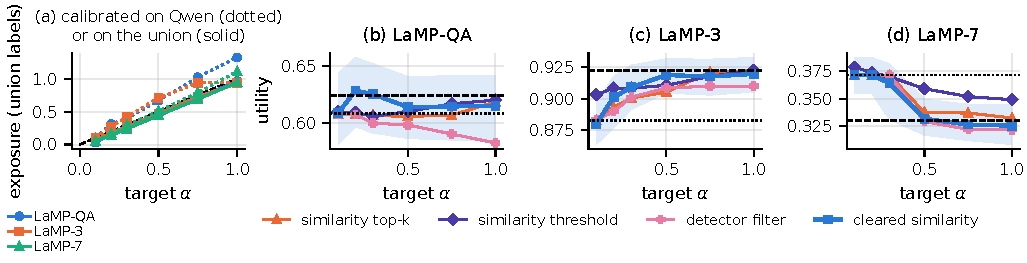
\includegraphics[width=\textwidth]{generated/fig_main.pdf}
\caption{(a) Exposure under union labels of test users, worst of four rules,
for rules calibrated on the primary auditor (dotted) or on the union
(solid). (b--d) Cross-fitted utility of the rules calibrated on union labels,
with a 95\% band for cleared similarity. Dotted is no profile, dashed top-5.}
\Description{Four panels show exposure versus the target and task utility
versus the target for four admission rules. Union calibration reduces measured
exposure; the utility cost varies across the three tasks.}
\label{fig:main}
\end{figure*}

\section{Risk-Controlled Record Admission}
\label{sec:method}

\paragraph{Threat model.}
A user's profile $P$ of personal records stays on the device, together with
a retriever, the admission rule and its scores. For a query $q$ the rule
places a set $A(q,P)$ of at most $K$ records from a candidate pool $C(q,P)$
in the prompt of a reader LLM run by a remote provider. Whatever is admitted
leaves the device, and the provider is assumed to see the full prompt. The
utility $U(q,S)$ of a set $S$ is the task metric of the reader's output.

\paragraph{Exposure.}
An \emph{auditor} sets $a(r)=1$ when record $r$ contains a self-disclosure,
a statement revealing personal information about the author or a person close
to them~\cite{dou2024reducing}. We control two losses of an admitted set, the
count $E(S)=\sum_{r\in S}a(r)\in[0,K]$ and the indicator
$Z(S)=\mathbb{1}[E(S)\ge1]$ that the prompt carries any disclosure. The
auditor may be a large model or a human annotator. It labels a sample of
consenting calibration users offline and never runs on the device.
This is incremental profile exposure, excluding the query sent by every
rule, even the empty rule. Counting a query as one additional record gives
$E_{\rm total}=E(S)+a(q)$ and only $\mathbb{E}E_{\rm total}\le\alpha+1$
without a query audit. A total-prompt budget needs query labels and an
abstention or local-only fallback.

\paragraph{Admission families.}
We calibrate any family $\{A_\lambda\}$ with an ordered parameter on a finite
grid $\lambda_0<\dots<\lambda_J$ and $A_{\lambda_0}=\emptyset$. A
\emph{top-$k$} rule admits the $k$ highest-scoring candidates. A
\emph{threshold} rule admits up to $K$ candidates whose score is at least a
cut-off that decreases along the grid, so the number of records adapts to
the query. A \emph{cleared} rule uses an on-device sensitivity proxy
$s(r)\in[0,1]$ and admits
\begin{equation}
A_\lambda(q,P)=\operatorname{top}\text{-}K_{g}\,\{r\in C(q,P): s(r)\le\lambda\},
\label{eq:gate}
\end{equation}
where $g$ ranks candidates, by similarity to $q$ in our main rule. Top-$k$
and threshold rules are nested. In a cleared rule a newly cleared record can
displace a less highly ranked one, so we control the running maximum
$L(\lambda_j)=\max_{j'\le j}\ell(A_{\lambda_{j'}})$ of the loss $\ell\in\{E,Z\}$,
which is nondecreasing, bounded by $B=K$ for $E$ and $B=1$ for $Z$, and never
below $\ell$.

\paragraph{Calibration.}
Let $L_1,\dots,L_n$ be the loss curves of $n$ audited calibration users and
$\hat R_n(\lambda)=\frac1n\sum_i L_i(\lambda)$. For a target $\alpha$ we deploy
\begin{equation}
\hat\lambda=\max\Bigl\{\lambda_j:\ \tfrac{n}{n+1}\hat R_n(\lambda_j)+\tfrac{B}{n+1}\le\alpha\Bigr\},
\label{eq:crc}
\end{equation}
and $\hat\lambda=\lambda_0$ when no grid point qualifies.

\begin{proposition}[Exposure control~{\cite[Thm.~1]{angelopoulos2024conformal}}]
\label{prop:cert}
Suppose the grid, the family and its scores are fixed using users independent
of the calibration and test users, and the $n$ calibration users and a new
user are exchangeable. Then
\[
\mathbb{E}\bigl[\ell(A_{\hat\lambda}(q_{n+1},P_{n+1}))\bigr]\le\alpha.
\]
\end{proposition}

This is conformal risk control with the direction of monotonicity flipped, and
we claim no new theory (proof and a synthetic check in the artifact). What the
tool adds to data minimization is a single, rule-agnostic way to set how much a
gate may admit. The exchangeable unit is the user. A poor ranking lowers
$\hat\lambda$ and utility while the bound still holds. Auditing one fixed rule
with a confidence bound is the one-point grid, which can only pass or fail.
For independent calibration users from the deployment distribution,
Learn-then-Test~\cite{angelopoulos2025learn} gives probability $1-\delta$
over the calibration draw, using
Hoeffding--Bentkus p-values~\cite{bates2021distribution}, testing grid points
in increasing order. Because a bound on labels $a'$ implies a bound on any
labels $a\le a'$, calibrating on the union of several auditors' labels
bounds the exposure measured by each of them.

\paragraph{Minimality gap.}
Within the top-8 candidates $C_8$, the minimal sufficient set
$S^\star_\varepsilon=\arg\min\{E(S): S\subseteq C_8,\ U(q,S)\ge U(q,C)-\varepsilon\}$
is the least exposing set that keeps the utility of the whole pool within
$\varepsilon$, and the minimality gap of a rule is
$\mathbb{E}[E(A)]-\mathbb{E}[E(S^\star_\varepsilon)]$. Minimality refers to auditor-flagged records only, never to all personal data
in a prompt. We approximate $S^\star_\varepsilon$ by greedy extensions of up to
three records scored against the gold output, a hindsight reference no
deployable rule can match.

\begin{table*}[t]
\caption{Cross-fitted union-flagged exposure, records and utility at $\alpha=0.2$.
CRC controls expected risk; LTT controls population risk with probability
$1-\delta$ over calibration draws. Marks $^{-}$/$^{+}$ denote loss/gain
against top-5 at 90\%, $\dagger$ denotes non-inferiority. All groups use the 7B reader; 14B results are in the supplement.}
\label{tab:main}
\small
\setlength{\tabcolsep}{3.2pt}
\begin{tabular}{lrrrrrrrrr}
\toprule
 & \multicolumn{3}{c}{LaMP-QA} & \multicolumn{3}{c}{LaMP-3} & \multicolumn{3}{c}{LaMP-7} \\
\cmidrule(lr){2-4} \cmidrule(lr){5-7} \cmidrule(lr){8-10}
Admission rule & Exp. & Rec. & Util. & Exp. & Rec. & Util. & Exp. & Rec. & Util. \\
\midrule
\multicolumn{10}{l}{\emph{Uncalibrated, whole records}} \\
No profile & 0.00 & 0.0 & 0.608 & 0.00 & 0.0 & 0.883 & 0.00 & 0.0 & 0.372 \\
Similarity top-5 & 1.41 & 5.0 & 0.624 & 0.94 & 5.0 & 0.922 & 2.06 & 5.0 & 0.330 \\
Detector filter top-5 & 0.68 & 3.8 & 0.582 & 0.52 & 4.0 & 0.910 & 1.65 & 4.5 & 0.322 \\
\midrule
\multicolumn{10}{l}{\emph{Uncalibrated, rating summaries or text removal}} \\
Ratings only & -- & -- & -- & 0.00 & 5.0 & 0.913 & -- & -- & -- \\
Redact detector-flagged text & -- & -- & -- & 0.42 & 5.0 & 0.921$^{\dagger}$ & -- & -- & -- \\
Redact auditor-flagged text & -- & -- & -- & 0.00 & 5.0 & 0.921$^{\dagger}$ & -- & -- & -- \\
Mean past rating only & -- & -- & -- & 0.00 & 0.0 & 0.893$^{-}$ & -- & -- & -- \\
\midrule
\multicolumn{10}{l}{\emph{Calibrated on union labels, $\mathbb{E}$-bound at $\alpha=0.2$ (Eq.~2)}} \\
Similarity top-$k$ & 0.00 & 0.0 & 0.608 & 0.10 & 0.5 & 0.893$^{-}$ & 0.00 & 0.0 & 0.372$^{+}$ \\
Similarity threshold & 0.21 & 0.5 & 0.609 & 0.17 & 1.3 & 0.908$^{-}$ & 0.14 & 0.4 & 0.374$^{+}$ \\
Detector filter & 0.02 & 0.1 & 0.607 & 0.11 & 1.0 & 0.890$^{-}$ & 0.00 & 0.0 & 0.372$^{+}$ \\
Cleared similarity & 0.13 & 2.2 & 0.628 & 0.15 & 3.1 & 0.901$^{-}$ & 0.00 & 0.0 & 0.372$^{+}$ \\
\midrule
\multicolumn{10}{l}{\emph{Calibrated on union labels, per-draw bound at $\alpha=0.2$, $\delta=0.1$}} \\
Similarity top-$k$ & 0.00 & 0.0 & 0.608 & 0.00 & 0.0 & 0.883$^{-}$ & 0.00 & 0.0 & 0.372$^{+}$ \\
Similarity threshold & 0.04 & 0.1 & 0.609 & 0.08 & 0.5 & 0.903$^{-}$ & 0.04 & 0.1 & 0.378$^{+}$ \\
Detector filter & 0.00 & 0.0 & 0.608 & 0.00 & 0.0 & 0.883$^{-}$ & 0.00 & 0.0 & 0.372$^{+}$ \\
Cleared similarity & 0.00 & 0.0 & 0.608 & 0.05 & 1.8 & 0.880$^{-}$ & 0.00 & 0.0 & 0.372$^{+}$ \\
\bottomrule
\end{tabular}

\end{table*}

\section{Experimental Setup}
\label{sec:setup}
\paragraph{Tasks and users.}
We use three tasks with real user profiles and one query per user.
LaMP-QA~\cite{salemi2025lampqa} (Lifestyle and Personal Development,
validation) asks for a long answer to a user's question given the user's
earlier posts and scores the share of user-specific rubric aspects the answer
addresses. LaMP-3 (product rating) and LaMP-7 (tweet
paraphrasing)~\cite{salemi2024lamp}, user-based dev splits, are scored by
$1-|\text{error}|/4$ and ROUGE-L. Per task, deduplicated users are drawn in a
fixed random order: 120 training users fit the scores and grids, disjoint
evaluation users are audited (\qaNEval{}, \threeNEval{} and \sevenNEval{}),
and \qaNReader{}, \threeNReader{} and \sevenNReader{} of them receive reader
calls for every candidate set. Validity is measured over 1000 random halvings into calibration and test
users, utility by 2-fold cross-fitting over 200 partitions with user-bootstrap
intervals. No test user touches a score, a grid or a threshold.

\paragraph{Labels and models.}
Two auditors label every top-8 candidate with the self-disclosure taxonomy of
Dou et al.~\cite{dou2024reducing} (19 categories merged into 14),
Qwen2.5-7B-Instruct and Gemma-2-9B, one call per record. A record counts as
flagged when either auditor flags it, and these \emph{union labels} are used
for calibration and for every exposure we report unless stated. No human
labels exist. The reader is Qwen2.5-7B-Instruct (4-bit, greedy), standing in
for the provider's model, with Qwen2.5-14B on the first \FourteenN{} LaMP-3
users and Llama-3.1-8B on the first \threeLlamaN{} as second readers. For
LaMP-QA, Qwen-7B applies the benchmark rubric; Gemma-2-9B independently
rescores all 3,184 saved answers for 150 users as a judge-sensitivity check.
Both are model judgments.
Candidates are the 20 records most similar to the query under a MiniLM
encoder, rules choose among the top 8, and $K=5$.

\paragraph{Rules, baselines and tests.}
\emph{Similarity top-$k$} and \emph{similarity threshold} rank by encoder
similarity. The \emph{detector filter} drops records flagged by
Presidio~\cite{presidio2026software} entities or a small disclosure lexicon,
both written before any audit, and ranks the rest by similarity. The
\emph{cleared similarity} rule is Eq.~\eqref{eq:gate} with a logistic
sensitivity proxy on the MiniLM embedding and detector counts, fitted to the
Qwen auditor's labels of training users. Rules built on a learned necessity score are omitted because the score was
near random. On LaMP-3, where each record carries the user's past rating,
we compare the full-history mean rating alone and three field-level baselines that send the top-5 records with ratings
only, with the text of detector-flagged records removed, or with the text of
union-flagged records removed, the last an upper reference no on-device gate
can compute. Where top-5 beats no profile, we report the plug-in share of its
gain a rule keeps with a user-bootstrap interval, and call a rule
non-inferior when the lower 90\% bound of that share exceeds 75\%, a margin
fixed before the 14B run. All significance marks and corresponding loss/gain claims use two-sided 90\% intervals; descriptive effect intervals use 95\%. A rule whose 90\% interval of the difference to
top-5 lies below zero is a significant loss. Cleared similarity at
$\alpha=0.5$ and $\alpha=0.2$ with every reader are the pre-specified
confirmatory cells, and the remaining rule-by-target cells are exploratory
and not corrected for multiplicity. The oracle searches up to three records
with $\varepsilon=0.05$ on \threeOrN{} users per task, using the Qwen labels
during the search and union labels in the reported exposure.

\section{Results}
\label{sec:results}

\paragraph{The guarantee is only as good as the auditor.}
The two auditors flag \qaRateDisc\% and \qaRateGemma\% (LaMP-QA),
\threeRateDisc\% and \threeRateGemma\% (LaMP-3) and \sevenRateDisc\% and
\sevenRateGemma\% (LaMP-7) of the top-8 candidates, with Cohen's $\kappa$ of
\qaKappaFull{}, \threeKappaFull{} and \sevenKappaFull{}, and the primary
auditor finds only \qaQwenRecGemma\%, \threeQwenRecGemma\% and
\sevenQwenRecGemma\% of the records the second one flags. Similarity top-5
places \qaESimK{}, \threeESimK{} and \sevenESimK{} union-flagged records in an
average prompt. Rules calibrated on the primary auditor stay below $\alpha$ under its own
labels, but under the second auditor's labels their mean exposure exceeds
$\alpha$ in up to \qaCalQwenMeasGemma\% of (target, rule) cells and under the
union in up to \qaCalQwenMeasUnion\% (Figure~\ref{fig:main}a). Calibrating on
the union (Table~\ref{tab:audit}) removes every excess under all three label
sources, as it must. Single calibration draws still exceed the
target in up to \CrcAboveMax\% of cases, because the bound holds in
expectation, while Learn-then-Test at $\delta=0.1$ keeps the share of draws
above the target at or below \LttAboveMax\%. Without human labels the bound
is relative to two small LLM auditors.

\begin{table}[t]
\caption{Share of the 24 (target, rule) cells whose mean test exposure
exceeds $\alpha$, with the largest excess in records, by calibration labels
and measurement labels.}
\label{tab:audit}
\small
\setlength{\tabcolsep}{3pt}
\begin{tabular}{llrrr}
\toprule
 & Calibrated on & \multicolumn{3}{c}{Measured with} \\
\cmidrule(lr){3-5}
Task & & Qwen & Gemma & Union \\
\midrule
LaMP-QA & Qwen & 0\% (-0.03) & 54\% (+0.16) & 67\% (+0.33) \\
 & Union & 0\% (-0.08) & 0\% (-0.05) & 0\% (-0.04) \\
LaMP-3 & Qwen & 0\% (-0.02) & 54\% (+0.12) & 62\% (+0.21) \\
 & Union & 0\% (-0.04) & 0\% (-0.03) & 0\% (-0.02) \\
LaMP-7 & Qwen & 0\% (-0.04) & 0\% (-0.06) & 17\% (+0.11) \\
 & Union & 0\% (-0.06) & 0\% (-0.06) & 0\% (-0.05) \\
\bottomrule
\end{tabular}

\end{table}

\paragraph{What the dial costs.}
Among the three main tasks, records help only on LaMP-3, where top-5 gains \threeTopFiveGain{} over no
profile with the 7B reader, \FourteenGain{} with the 14B reader and
\threeLlamaGain{} with Llama-3.1-8B (95\% intervals). There, a target of
$\alpha=0.2$ has a real cost. All four calibrated rules lose significantly
against top-5 with every reader (Table~\ref{tab:main}), and the best keeps
\threeSimThrKeptB{} of the 7B gain and \FourteenCSimKeptB{} of the 14B
gain. At $\alpha=0.5$ cleared similarity admits \FourteenCSimExpoD{} instead of
\FourteenESimK{} flagged records per prompt. It keeps \FourteenCSimKeptD{} of
the 14B gain, which passes our non-inferiority margin (lower 90\% bound
\FourteenCSimKeptLowD{}), and \threeCSimKeptD{} of the 7B gain, which is not
significantly below top-5 but does not pass it. The per-draw variant keeps \threeLttSimThrKeptB{} of the 7B gain at
$\alpha=0.2$. On LaMP-QA, top-5 does not beat no profile under Qwen (\SecondJudgeQwenGain{})
or Gemma (\SecondJudgeGain{}; 95\% intervals). Some rule comparisons
change significance across judges (supplement). On LaMP-7 records mislead the reader, so
rules that admit fewer of them beat top-5 and none beats no profile. Auditing one fixed rule (top-1, top-5 or detector top-5) with a per-draw
bound ships it in \threeFixLttDep\% of LaMP-3 draws at $\alpha=0.2$, whereas a
calibrated rule always ships its most permissive safe setting. The 14B table and LaMP-2 pilot are in the supplement.

The mean past rating alone retains \MeanRatingKept{} of the 7B gain
(90\% interval), below top-5 by \MeanRatingDelta{}.
This statistic contains personal information despite sending no record text.

\paragraph{Exposure needed and exposure under shift.}
The hindsight oracle keeps utility within $\varepsilon$ for \qaOrSuff\%,
\threeOrSuff\% and \sevenOrSuff\% of users, the empty set alone suffices for
\qaOrEmpty\%, \threeOrEmpty\% and \sevenOrEmpty\%, and the oracle admits a
flagged record for only \qaOrNeeds\%, \threeOrNeeds\% and \sevenOrNeeds\% of
users. The minimality gap of top-5 (\qaOrSimKGap{}, \threeOrSimKGap{} and
\sevenOrSimKGap{} records) is therefore almost its whole exposure: these
tasks rarely need a disclosing record. Calibrating on users with short profiles and testing on long ones, or the
reverse, exceeds $\alpha$ by up to \qaShiftMain{}, \threeShiftMain{} and
\sevenShiftMain{} records for our four rules, against at least
\qaShiftRand{} below $\alpha$ for random splits of the same size. Calibrating
separately in bins fixed by the training median keeps mean test exposure
below $\alpha$, given exchangeability within each bin. Rules
built on our necessity score, whose cross-validated Spearman correlation with
counterfactual gains is only \qaNecSpearman{}, \threeNecSpearman{} and
\sevenNecSpearman{}, fail worse under shift (up to \sevenShiftNec{} on
LaMP-7) and never beat similarity.

An illustrative severity sensitivity assigns weight 2 to health, mental-health,
sexual-orientation, race/nationality or finance flags and 1 to other flags.
At $\alpha=0.2$, recalibrated cleared similarity on LaMP-3 admits
\threeWeightedSize{} records at weighted loss \threeWeightedLoss{}, versus
\threeCountSize{} records at count loss \threeCountLoss{} (300 splits).
These policy weights are not a validated harm scale; full results are in the supplement.

\section{Related Work}
\label{sec:related}
Data minimization has been operationalized for recommendation by measuring
how much user data a model needs~\cite{biega2020operationalizing} and
formalized for learning as a constraint on retained
data~\cite{ganesh2025data}. For LLM prompts, Zhou et
al.~\cite{zhou2026operationalizing} search for the least disclosing variant of
one prompt, AirGapAgent~\cite{bagdasarian2024airgapagent}, SP-Mem~\cite{wang2026spmem}
and MemPrivacy~\cite{chen2026memprivacy} decide which personal fields a task
needs, PAPILLON~\cite{li2025papillon} and Salemi and
Zamani~\cite{salemi2026improving} split work between a local and a remote
model, MINIM~\cite{yu2026minim} scores necessity and sensitivity with fixed
thresholds, and Platnick et al.~\cite{platnick2025structured} select
data-minimal facts by submodular maximization. PURPLE~\cite{du2026purple} and
ENOUGH~\cite{liu2026enough} learn profile selection on LaMP~\cite{salemi2024lamp}.
Our cleared rule adds a calibrated exposure threshold to MINIM's design;
the oracle extends minimal-profile comparisons to audited record sets.
Conformal risk control and Learn-then-Test~\cite{angelopoulos2024conformal,bates2021distribution,angelopoulos2025learn}
have certified generation risk in RAG~\cite{kang2024crag},
factuality~\cite{mohri2024language,quach2024conformal}, harm and cost
trade-offs~\cite{overman2025conformal,laufer2023pareto}, agent
actions~\cite{feng2026cora,rahman2026beyond} and re-identification
audits~\cite{huang2026conformal}. Closest are CORA~\cite{feng2026cora}, which
gates agent actions with privacy as one harm, and Chakraborty et
al.~\cite{chakraborty2026principled}, who keep retrieved RAG context above a
lower bound on relevance, the mirror image of our upper bound on admitted
sensitive content. Our record-count exposure excludes joint inferences~\cite{staab2024beyond} and contextual norms studied by ConfAIde~\cite{mireshghallah2024confaide},
PrivacyLens~\cite{shao2024privacylens} and AgentDAM~\cite{zharmagambetov2025agentdam}.

\section{Conclusion}
\label{sec:conclusion}
A calibrated admission parameter bounds expected profile exposure under
auditor and exchangeability assumptions. On LaMP-3, strict targets cost
utility; a looser target retains most gain with less than half the top-5
exposure. Human validation remains open. Cumulative distinct disclosures
under real multi-query histories are not measured.

\section*{Ethical Considerations}
The method reduces the personal data a personalized assistant sends to a
model provider and makes the residual exposure a quantity a deployer can set
and verify. Its limits must be stated with it. The bound covers what the
auditors flag, our auditors are two small LLMs, and no human labels exist, so
a human audit of the calibration sample is needed before any deployment. The
bound is an expectation over users exchangeable with the calibration sample,
individual users can be exposed more than $\alpha$, and it covers one prompt
per user. Summing marginal bounds gives $T\alpha$ for expected cumulative
record occurrences only if every prompt satisfies the calibration assumptions.
Distinct disclosures are at most this sum, but this is neither a per-user
guarantee nor validation for adaptive queries, which we do not measure.
The guarantee can fail when
deployment users differ from calibration users. A
small $\alpha$ is a quantity of leakage and never an absence of it,
record-level labels miss inferences drawn from several records, and the
user's own query, which is always sent, is outside the measure. Calibration
requires that an auditor read the records of calibration users, who must
consent under a data agreement that deployment users do not need. We use only
existing public research benchmarks (LaMP under CC BY-NC-SA with source
licences, LaMP-QA with no declared licence over StackExchange posts that
StackExchange distributes under CC BY-SA) and recruit no participants. The
per-record labels we derive mark health, finance, sexual orientation and
other disclosures of real, pseudonymous authors and can be joined back to the
public benchmarks, so we treat them as sensitive derived data and will not
release them, nor any benchmark text or cached prompt. The released artifact
therefore reproduces the tables from the labels only by re-running the
auditors on the public benchmarks, and lists what it excludes. A deployed system must obtain consent
for retaining personal history and honor deletion, and a score is no
substitute for user control over what is shared.

\bibliographystyle{ACM-Reference-Format}
\bibliography{references}
\end{document}
